\section{Thiết kế hệ thống}

Phần mềm ``Quản lí bệnh án bệnh nhân" - \textbf{MeReMa} được thiết dựa trên kiến trúc 3 lớp, với các lớp lần lượt là: presentation layer (client), business layer (server) và data layer (database). Khi này, server sẽ đảm nhiệm phần lớn các tác vụ xử lý dữ liệu và logic nghiệp vụ, trong khi client chủ yếu chỉ cần hiển thị thông tin lên giao diện người dùng và gửi yêu cầu đến máy chủ để truy xuất thông tin, và database nhận nhiệm vụ lưu trữ thông tin.
\begin{itemize}
  \item Ưu điểm:
    \begin{itemize}
      \item Đơn giản trong việc triển khai, vì phần lớn logic nghiệp vụ được xử lý trên máy chủ.
      \item Dễ dàng mở rộng và bảo trì, vì các thay đổi trong logic nghiệp vụ chỉ cần thực hiện trên máy chủ mà không ảnh hưởng đến client.
      \item Giảm tải cho client, vì client chỉ cần gửi yêu cầu và nhận dữ liệu từ máy chủ.
      \item Luồng dữ liệu rõ ràng, dễ dàng quản lý và bảo mật thông tin.
    \end{itemize}
  \item Nhược điểm:
    \begin{itemize}
      \item Phụ thuộc vào máy chủ, nếu máy chủ gặp sự cố, toàn bộ hệ thống sẽ bị ảnh hưởng.
      \item Tải trọng trên máy chủ có thể tăng cao nếu có nhiều client cùng truy cập đồng thời.
      \item Yêu cầu kết nối mạng liên tục, nếu mất kết nối, client sẽ không thể truy cập dữ liệu.
    \end{itemize}
\end{itemize}

Dưới dây là sơ đồ kiến trúc hệ thống của phần mềm MeReMa:

\begin{figure}[H]
  \centering
  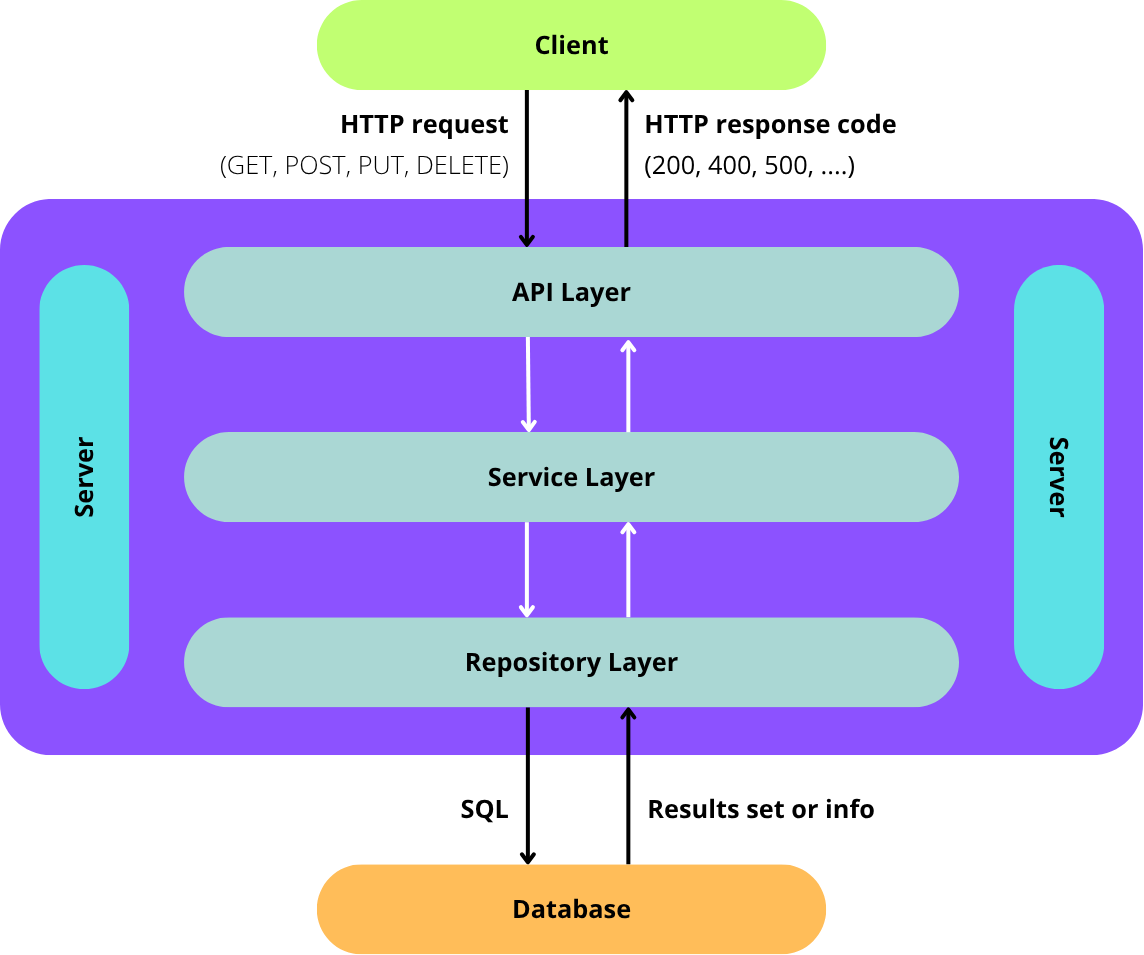
\includegraphics[width=0.8\textwidth]{src/figures/sys_arch.png}
  \caption{Sơ đồ kiến trúc hệ thống MeReMa}
  \label{fig:sys_arch}
\end{figure}

\subsection{Presentation Layer (Client)}

Lớp trình bày (presentation layer), được xem như \textbf{Client} của phần mềm MeReMa được xây dựng bằng ngôn ngữ lập trình \textbf{Dart}, sử dụng framework \textbf{Flutter} để phát triển ứng dụng desktop. Lớp này chịu trách nhiệm hiển thị giao diện người dùng và xử lý các tương tác của người dùng với phần mềm. Các thành phần chính của lớp này bao gồm:
\begin{itemize}
  \item Giao diện người dùng: Hiển thị các thông tin về bệnh nhân, bệnh án, lịch sử khám chữa bệnh, v.v. Giao diện được thiết kế thân thiện và dễ sử dụng, với các thành phần như danh sách bệnh nhân, biểu mẫu nhập liệu,
    nút chức năng, v.v.
  \item Xử lý sự kiện: Nhận các sự kiện từ người dùng như nhập liệu, nhấn nút, chọn mục trong danh sách, v.v. và gửi các yêu cầu tương ứng đến máy chủ để xử lý.
  \item Kết nối với máy chủ: Sử dụng HTTP hoặc WebSocket để gửi yêu cầu đến máy chủ và nhận dữ liệu trả về. Lớp này sẽ gửi các yêu cầu như đăng nhập, đăng ký, truy xuất thông tin bệnh nhân, cập nhật bệnh án, v.v. đến máy chủ và nhận dữ liệu trả về để hiển thị trên giao diện người dùng.
\end{itemize}

\subsection{Business Layer (Server)}

Lớp nghiệp vụ (business layer), được xem như \textbf{Server} của phần mềm MeReMa được xây dựng bằng ngôn ngữ lập trình \textbf{Golang}, sử dụng framework \textbf{Gin} để phát triển API và những thư viện khác nhằm mục đích xử lí dữ liệu, đồng thời tương tác với client và database. Lớp này chịu trách nhiệm xử lý các yêu cầu từ lớp trình bày, thực hiện các logic nghiệp vụ và tương tác với database; hoặc ngược lại, truy xuất thông tin từ database, xử lí rồi trả về cho client. Các thành phần chính của lớp này bao gồm:
\begin{itemize}
  \item Lớp API (API layer): Cung cấp các endpoint để client có thể gửi yêu cầu và nhận dữ liệu. Các endpoint này bao gồm đăng nhập, đăng ký, truy xuất thông tin bệnh nhân, cập nhật bệnh án, v.v. được xây dựng dựa trên RESTful API, với các phương thức như GET, POST, PUT, DELETE để tương tác với dữ liệu.
  \item Lớp dịch vụ (Service layer): Xử lý các logic nghiệp vụ như xác thực người dùng, kiểm tra quyền truy cập, xử lý dữ liệu bệnh nhân, v.v. Lớp này sẽ nhận các yêu cầu từ client sau khi qua lớp API, thực hiện các logic nghiệp vụ cần thiết, để yêu cầu lớp lưu trữ lưu dữ liệu vào database hoặc truy xuất dữ liệu từ database rồi xử lí dữ liệu và trả về lớp API.
  \item Lớp lưu trữ (Repository layer): Tương tác với database để lưu trữ và truy xuất dữ liệu. Lớp này sẽ sử dụng driver database để kết nối với database, thực hiện các truy vấn SQL để tương tác với dữ liệu. Lớp này sẽ nhận các yêu cầu từ lớp dịch vụ, thực hiện các truy vấn cần thiết và trả về kết quả cho lớp dịch vụ.
\end{itemize}

\subsection{Data Layer (Database)}

Lớp dữ liệu (data layer), được xem như \textbf{Database} của phần mềm MeReMa được xây dựng dựa trên hệ quản trị cơ sở dữ liệu \textbf{PostgreSQL}, với các bảng lưu trữ thông tin về người dùng, bệnh nhân, bệnh án, bệnh án, v.v. Lớp này chịu trách nhiệm lưu trữ và quản lý dữ liệu của phần mềm. Các thành phần chính của lớp này bao gồm:
\begin{itemize}
  \item Các bảng dữ liệu: Lưu trữ các thông tin về người dùng, bệnh nhân, bệnh án, lịch sử khám chữa bệnh, v.v. Mỗi bảng sẽ có các trường dữ liệu tương ứng để lưu trữ thông tin cần thiết.
  \item Quan hệ giữa các bảng: Thiết lập các quan hệ giữa các bảng để đảm bảo tính toàn vẹn của dữ liệu.
  \item Các ràng buộc dữ liệu: Đảm bảo tính nhất quán và toàn vẹn của dữ liệu, ví dụ như ràng buộc khóa chính, khóa ngoại, ràng buộc duy nhất, v.v.
  \item Các chỉ mục (index): Tăng tốc độ truy vấn dữ liệu bằng cách tạo các chỉ mục trên các trường dữ liệu thường xuyên được truy vấn.
\end{itemize}